\section{Data Application}\label{sec:data}

The data in our example represent the orientations of cubic crystals on a Nickel surface measured by electron backscatter diffraction. The data were obtained using a 14-fold technical replicate in each location. 
A central interest in EBSD data is the identification of so-called {\it grain maps} -- grains are defined as regions on the surface with nearly identical main direction $\bm S$. This makes the estimation of $\bm S$ crucial to the field. 

%After applying all four of our estimators to each location on the surface, we found -- surprisingly -- large differences between the estimates in some of the locations. 
%Figure \ref{fig:eyeballs-1} shows sphere plots of the data and the estimates for one of these locations.  Because rotation matrices are orthogonal, each of their columns (and rows) represents elements on the unit sphere.  Note that the figure shows a sample of a single location, yet the clustering in the data suggests very clearly the presence of \emph{two} main directions. When combining data from multiple locations, see Figure \ref{fig:eyeballs}, we find the same two main directions, independent of location. The \emph{within  location variability} of the estimates of $\bm S$ is much higher than the \emph{between location variability}. 

Figure \ref{fig:eyeballs} shows sphere plots of  data and the estimates for seven randomly chosen locations within a single grain.  Because rotation matrices are orthogonal, each of their columns (and rows) represents elements on the unit sphere. The sphere plots indicate some clustering in the data suggesting the presence of \emph{several} main directions. 

The projected median $\widetilde{\bm S}_P$ is the only estimator that is not affected by this clustering in the sample. $\widetilde{\bm S}_P$ identifies the main direction of the largest group within the sample.


%\begin{figure}[htbp] %  figure placement: here, top, bottom, or page
%   \centering
%   \includegraphics[width=.325\textwidth]{images/eyeball-1-1.pdf} 
%   \includegraphics[width=.325\textwidth]{images/eyeball-1-2.pdf} 
%   \includegraphics[width=.325\textwidth]{images/eyeball-1-3.pdf} 
%   \caption{Sphere plots of EBSD measurements at a single location. The data sample is shown as dark grey points, the estimates of the main direction are colored and labelled. The clustering of the results makes the existence  of two main directions  quite obvious. }
%   \label{fig:eyeballs-1}
%\end{figure}
%

\begin{figure}[htbp] %  figure placement: here, top, bottom, or page
   \centering
   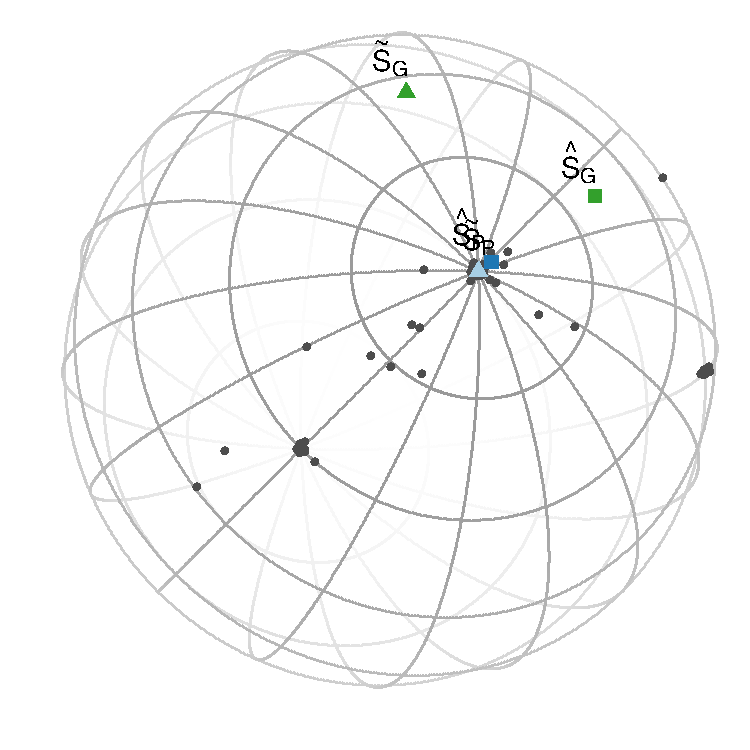
\includegraphics[width=.325\textwidth]{images/eyeball-7-1.pdf} 
   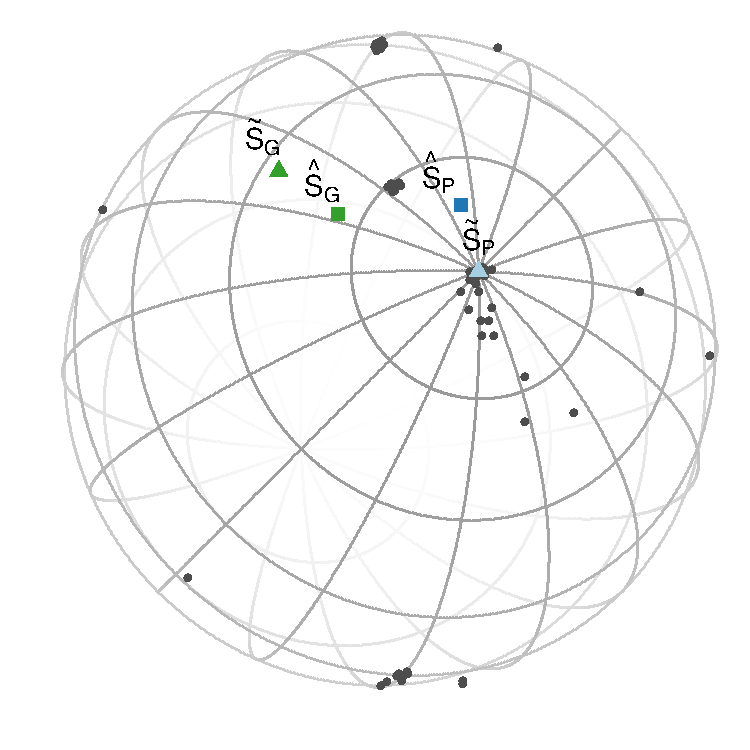
\includegraphics[width=.325\textwidth]{images/eyeball-7-2.pdf} 
   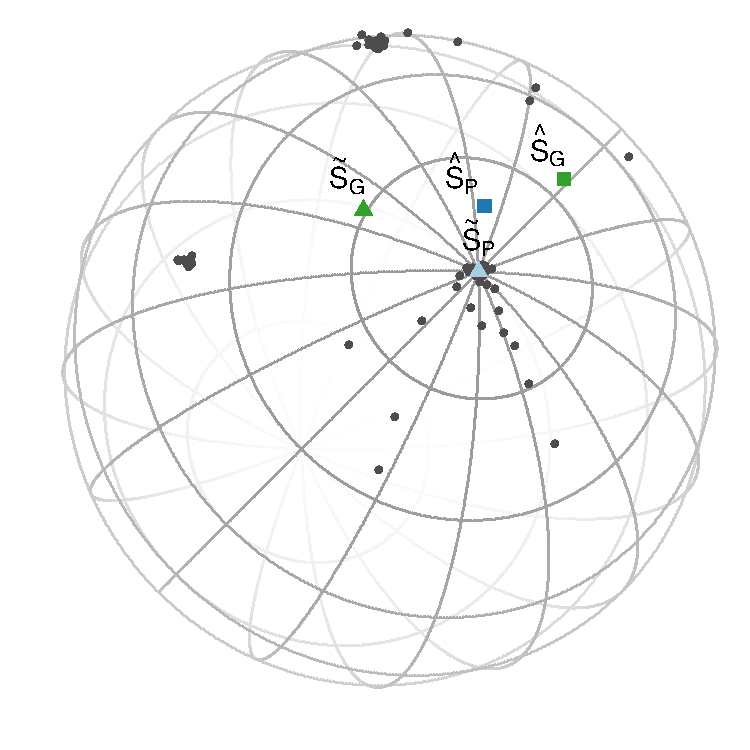
\includegraphics[width=.325\textwidth]{images/eyeball-7-3.pdf} 
   \caption{Sphere plots of EBSD measurements. The sample ($n=98$) is taken from seven locations from within what was thought to be a single grain, but the data suggest the existence of several -- very stable -- main directions, as can be seen by the distinct grouping. The projected median $\widetilde{\bm S}_P$ is located in the center of the largest cluster of points.}
   \label{fig:eyeballs}
\end{figure}

Histograms of mis-orientation angles between each rotation in the sample and each of the four estimates of $\bm S$ are shown in Figure \ref{fig:histograms}. The distribution of the mis-orientation angles depends greatly on the choice of estimator. The only estimator with a large group of small mis-orientation angles is $\widetilde{\bm S}_P$, the projected median. However, the multiple spikes in the  histograms of mis-orientation angles for all of the estimators indicate a problem in estimating a single main direction. 


\begin{figure}[htbp] %  figure placement: here, top, bottom, or page
   \centering
%   \includegraphics[width=\textwidth]{images/histogram-20} 
   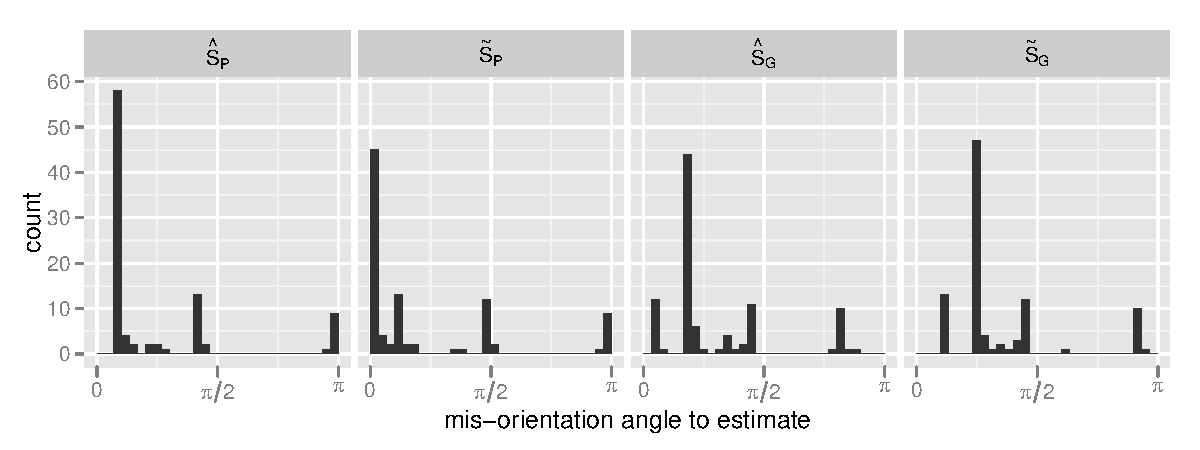
\includegraphics[width=\textwidth]{images/histogram-7} 
   \caption{Histograms of the mis-orientation angles between rotational sample and estimates for a sample of size  $n=98$, combining data from seven locations. Angles are highly influenced by the choice of metric and method. }
   \label{fig:histograms}
\end{figure}
